\section{Результаты измерений}

\[
    D = 45\;\text{мм}
\]
\[
    a = D/2
\]
\[
    h = 1{,}5\;\text{мм}
\]


\begin{table}[!ht]
    \centering
    \caption{Низкие частоты}
    \begin{tabular}{|l|l|l|l|l|}
\hline
$\nu,\;\text{Гц}$ & $V,\;\text{В}$ & $I,\;\text{мА}$ & $\xi,\;\text{В} / \text{Гц}\cdot\text{мА}$ & $H_1/H_2$\\\hline
$20{,}00 \pm 0{,}10$ & $\left(1389{,}0 \pm 1{,}0\right)\cdot 10^{-4}$ & $495{,}550 \pm 0{,}010$ & $\left(1401 \pm 7\right)\cdot 10^{-8}$ & $\left(1002 \pm 5\right)\cdot 10^{-3}$\\\hline
$30{,}00 \pm 0{,}10$ & $\left(2047{,}0 \pm 1{,}0\right)\cdot 10^{-4}$ & $492{,}800 \pm 0{,}010$ & $\left(1385 \pm 5\right)\cdot 10^{-8}$ & $\left(990 \pm 3\right)\cdot 10^{-3}$\\\hline
$40{,}00 \pm 0{,}10$ & $\left(2666{,}0 \pm 1{,}0\right)\cdot 10^{-4}$ & $488{,}080 \pm 0{,}010$ & $\left(1366 \pm 3\right)\cdot 10^{-8}$ & $\left(977 \pm 3\right)\cdot 10^{-3}$\\\hline
$50{,}00 \pm 0{,}10$ & $\left(3240{,}0 \pm 1{,}0\right)\cdot 10^{-4}$ & $482{,}240 \pm 0{,}010$ & $\left(1344 \pm 3\right)\cdot 10^{-8}$ & $\left(961 \pm 2\right)\cdot 10^{-3}$\\\hline
$60{,}00 \pm 0{,}10$ & $\left(3766{,}0 \pm 1{,}0\right)\cdot 10^{-4}$ & $475{,}740 \pm 0{,}010$ & $\left(1319 \pm 2\right)\cdot 10^{-8}$ & $\left(944 \pm 2\right)\cdot 10^{-3}$\\\hline
$70{,}00 \pm 0{,}10$ & $\left(4243{,}0 \pm 1{,}0\right)\cdot 10^{-4}$ & $468{,}820 \pm 0{,}010$ & $\left(1293 \pm 2\right)\cdot 10^{-8}$ & $\left(924{,}8 \pm 1{,}4\right)\cdot 10^{-3}$\\\hline
$80{,}00 \pm 0{,}10$ & $\left(4670{,}0 \pm 1{,}0\right)\cdot 10^{-4}$ & $461{,}730 \pm 0{,}010$ & $\left(1264 \pm 2\right)\cdot 10^{-8}$ & $\left(904{,}3 \pm 1{,}2\right)\cdot 10^{-3}$\\\hline
$90{,}00 \pm 0{,}10$ & $\left(5050{,}0 \pm 1{,}0\right)\cdot 10^{-4}$ & $454{,}680 \pm 0{,}010$ & $\left(1234{,}1 \pm 1{,}4\right)\cdot 10^{-8}$ & $\left(882{,}7 \pm 1{,}1\right)\cdot 10^{-3}$\\\hline
$100{,}00 \pm 0{,}10$ & $\left(5387{,}0 \pm 1{,}0\right)\cdot 10^{-4}$ & $447{,}810 \pm 0{,}010$ & $\left(1203{,}0 \pm 1{,}2\right)\cdot 10^{-8}$ & $\left(8604 \pm 9\right)\cdot 10^{-4}$\\\hline
$110{,}00 \pm 0{,}10$ & $\left(5684{,}0 \pm 1{,}0\right)\cdot 10^{-4}$ & $441{,}220 \pm 0{,}010$ & $\left(1171{,}1 \pm 1{,}1\right)\cdot 10^{-8}$ & $\left(8377 \pm 8\right)\cdot 10^{-4}$\\\hline
$120{,}00 \pm 0{,}10$ & $\left(5946{,}0 \pm 1{,}0\right)\cdot 10^{-4}$ & $434{,}940 \pm 0{,}010$ & $\left(1139{,}2 \pm 1{,}0\right)\cdot 10^{-8}$ & $\left(8149 \pm 8\right)\cdot 10^{-4}$\\\hline
\end{tabular}

\end{table}

\begin{table}[!ht]
    \centering
    \caption{Высокие частоты}
    \resizebox{\columnwidth}{!}{\begin{tabular}{|l|l|l|l|l|l|l|l|}
\hline
$\nu,\;\text{Гц}$ & $V,\;\text{В}$ & $I,\;\text{мА}$ & $\varphi$ & $T$ & $\xi,\;\text{В} / \text{Гц}\cdot\text{мА}$ & $\psi$ & $H_1/H_2$\\\hline
$120{,}0 \pm 1{,}0$ & $\left(5946{,}0 \pm 1{,}0\right)\cdot 10^{-4}$ & $\left(4349400{,}0 \pm 1{,}0\right)\cdot 10^{-4}$ & $2{,}80 \pm 0{,}05$ & $8{,}40 \pm 0{,}05$ & $\left(1139 \pm 9\right)\cdot 10^{-8}$ & $0{,}52 \pm 0{,}04$ & $\left(815 \pm 7\right)\cdot 10^{-3}$\\\hline
$170{,}0 \pm 1{,}0$ & $\left(6847{,}0 \pm 1{,}0\right)\cdot 10^{-4}$ & $\left(4081000{,}0 \pm 1{,}0\right)\cdot 10^{-4}$ & $2{,}20 \pm 0{,}05$ & $5{,}90 \pm 0{,}05$ & $\left(987 \pm 6\right)\cdot 10^{-8}$ & $0{,}77 \pm 0{,}06$ & $\left(706 \pm 4\right)\cdot 10^{-3}$\\\hline
$220{,}0 \pm 1{,}0$ & $\left(7327{,}0 \pm 1{,}0\right)\cdot 10^{-4}$ & $\left(3904800{,}0 \pm 1{,}0\right)\cdot 10^{-4}$ & $2{,}70 \pm 0{,}05$ & $4{,}60 \pm 0{,}05$ & $\left(853 \pm 4\right)\cdot 10^{-8}$ & $2{,}12 \pm 0{,}08$ & $\left(610 \pm 3\right)\cdot 10^{-3}$\\\hline
$270{,}0 \pm 1{,}0$ & $\left(7590{,}0 \pm 1{,}0\right)\cdot 10^{-4}$ & $\left(3783600{,}0 \pm 1{,}0\right)\cdot 10^{-4}$ & $3{,}10 \pm 0{,}05$ & $7{,}50 \pm 0{,}05$ & $\left(743 \pm 3\right)\cdot 10^{-8}$ & $1{,}03 \pm 0{,}05$ & $\left(531 \pm 2\right)\cdot 10^{-3}$\\\hline
$320{,}0 \pm 1{,}0$ & $\left(7735{,}0 \pm 1{,}0\right)\cdot 10^{-4}$ & $\left(3694500{,}0 \pm 1{,}0\right)\cdot 10^{-4}$ & $3{,}60 \pm 0{,}05$ & $6{,}30 \pm 0{,}05$ & $\left(654 \pm 2\right)\cdot 10^{-8}$ & $2{,}02 \pm 0{,}06$ & $\left(468{,}0 \pm 1{,}5\right)\cdot 10^{-3}$\\\hline
$370{,}0 \pm 1{,}0$ & $\left(7803{,}0 \pm 1{,}0\right)\cdot 10^{-4}$ & $\left(3625700{,}0 \pm 1{,}0\right)\cdot 10^{-4}$ & $2{,}70 \pm 0{,}05$ & $5{,}50 \pm 0{,}05$ & $\left(582 \pm 2\right)\cdot 10^{-8}$ & $1{,}51 \pm 0{,}06$ & $\left(416{,}0 \pm 1{,}1\right)\cdot 10^{-3}$\\\hline
$420{,}0 \pm 1{,}0$ & $\left(7839{,}0 \pm 1{,}0\right)\cdot 10^{-4}$ & $\left(3568900{,}0 \pm 1{,}0\right)\cdot 10^{-4}$ & $2{,}60 \pm 0{,}05$ & $4{,}80 \pm 0{,}05$ & $\left(523{,}0 \pm 1{,}2\right)\cdot 10^{-8}$ & $1{,}83 \pm 0{,}07$ & $\left(3741 \pm 9\right)\cdot 10^{-4}$\\\hline
$470{,}0 \pm 1{,}0$ & $\left(7844{,}0 \pm 1{,}0\right)\cdot 10^{-4}$ & $\left(3519300{,}0 \pm 1{,}0\right)\cdot 10^{-4}$ & $2{,}40 \pm 0{,}05$ & $4{,}30 \pm 0{,}05$ & $\left(474{,}2 \pm 1{,}0\right)\cdot 10^{-8}$ & $1{,}94 \pm 0{,}08$ & $\left(3392 \pm 7\right)\cdot 10^{-4}$\\\hline
$520{,}0 \pm 1{,}0$ & $\left(7824{,}0 \pm 1{,}0\right)\cdot 10^{-4}$ & $\left(3473700{,}0 \pm 1{,}0\right)\cdot 10^{-4}$ & $2{,}10 \pm 0{,}05$ & $3{,}90 \pm 0{,}05$ & $\left(4331 \pm 8\right)\cdot 10^{-9}$ & $1{,}81 \pm 0{,}09$ & $\left(3098 \pm 6\right)\cdot 10^{-4}$\\\hline
$570{,}0 \pm 1{,}0$ & $\left(7789{,}0 \pm 1{,}0\right)\cdot 10^{-4}$ & $\left(3430600{,}0 \pm 1{,}0\right)\cdot 10^{-4}$ & $1{,}80 \pm 0{,}05$ & $3{,}60 \pm 0{,}05$ & $\left(3983 \pm 7\right)\cdot 10^{-9}$ & $1{,}57 \pm 0{,}10$ & $\left(2849 \pm 5\right)\cdot 10^{-4}$\\\hline
$620{,}0 \pm 1{,}0$ & $\left(7743{,}0 \pm 1{,}0\right)\cdot 10^{-4}$ & $\left(3389000{,}0 \pm 1{,}0\right)\cdot 10^{-4}$ & $1{,}70 \pm 0{,}05$ & $3{,}20 \pm 0{,}05$ & $\left(3685 \pm 6\right)\cdot 10^{-9}$ & $1{,}77 \pm 0{,}11$ & $\left(2636 \pm 4\right)\cdot 10^{-4}$\\\hline
$670{,}0 \pm 1{,}0$ & $\left(7688{,}0 \pm 1{,}0\right)\cdot 10^{-4}$ & $\left(3348200{,}0 \pm 1{,}0\right)\cdot 10^{-4}$ & $3{,}60 \pm 0{,}05$ & $7{,}50 \pm 0{,}05$ & $\left(3427 \pm 5\right)\cdot 10^{-9}$ & $1{,}45 \pm 0{,}05$ & $\left(2451 \pm 4\right)\cdot 10^{-4}$\\\hline
$720{,}0 \pm 1{,}0$ & $\left(7628{,}0 \pm 1{,}0\right)\cdot 10^{-4}$ & $\left(3307300{,}0 \pm 1{,}0\right)\cdot 10^{-4}$ & $3{,}60 \pm 0{,}05$ & $7{,}00 \pm 0{,}05$ & $\left(3203 \pm 4\right)\cdot 10^{-9}$ & $1{,}66 \pm 0{,}05$ & $\left(2291 \pm 3\right)\cdot 10^{-4}$\\\hline
$770{,}0 \pm 1{,}0$ & $\left(7561{,}0 \pm 1{,}0\right)\cdot 10^{-4}$ & $\left(3267500{,}0 \pm 1{,}0\right)\cdot 10^{-4}$ & $3{,}40 \pm 0{,}05$ & $6{,}60 \pm 0{,}05$ & $\left(3005 \pm 4\right)\cdot 10^{-9}$ & $1{,}67 \pm 0{,}05$ & $\left(2150 \pm 3\right)\cdot 10^{-4}$\\\hline
$820{,}0 \pm 1{,}0$ & $\left(7488{,}0 \pm 1{,}0\right)\cdot 10^{-4}$ & $\left(3227400{,}0 \pm 1{,}0\right)\cdot 10^{-4}$ & $3{,}10 \pm 0{,}05$ & $6{,}20 \pm 0{,}05$ & $\left(2829 \pm 3\right)\cdot 10^{-9}$ & $1{,}57 \pm 0{,}06$ & $\left(2024 \pm 3\right)\cdot 10^{-4}$\\\hline
$870{,}0 \pm 1{,}0$ & $\left(7411{,}0 \pm 1{,}0\right)\cdot 10^{-4}$ & $\left(3187700{,}0 \pm 1{,}0\right)\cdot 10^{-4}$ & $2{,}90 \pm 0{,}05$ & $5{,}80 \pm 0{,}05$ & $\left(2672 \pm 3\right)\cdot 10^{-9}$ & $1{,}57 \pm 0{,}06$ & $\left(1911 \pm 2\right)\cdot 10^{-4}$\\\hline
$920{,}0 \pm 1{,}0$ & $\left(7331{,}0 \pm 1{,}0\right)\cdot 10^{-4}$ & $\left(3147600{,}0 \pm 1{,}0\right)\cdot 10^{-4}$ & $2{,}70 \pm 0{,}05$ & $5{,}50 \pm 0{,}05$ & $\left(2532 \pm 3\right)\cdot 10^{-9}$ & $1{,}51 \pm 0{,}06$ & $\left(1811 \pm 2\right)\cdot 10^{-4}$\\\hline
$970{,}0 \pm 1{,}0$ & $\left(7247{,}0 \pm 1{,}0\right)\cdot 10^{-4}$ & $\left(3107400{,}0 \pm 1{,}0\right)\cdot 10^{-4}$ & $5{,}20 \pm 0{,}05$ & $10{,}40 \pm 0{,}05$ & $\left(2404 \pm 3\right)\cdot 10^{-9}$ & $1{,}57 \pm 0{,}03$ & $\left(1720 \pm 2\right)\cdot 10^{-4}$\\\hline
$1020{,}0 \pm 1{,}0$ & $\left(7161{,}0 \pm 1{,}0\right)\cdot 10^{-4}$ & $\left(3067200{,}0 \pm 1{,}0\right)\cdot 10^{-4}$ & $4{,}90 \pm 0{,}05$ & $9{,}80 \pm 0{,}05$ & $\left(2289 \pm 2\right)\cdot 10^{-9}$ & $1{,}57 \pm 0{,}04$ & $\left(1637 \pm 2\right)\cdot 10^{-4}$\\\hline
$1070{,}0 \pm 1{,}0$ & $\left(7074{,}0 \pm 1{,}0\right)\cdot 10^{-4}$ & $\left(3026800{,}0 \pm 1{,}0\right)\cdot 10^{-4}$ & $4{,}70 \pm 0{,}05$ & $9{,}40 \pm 0{,}05$ & $\left(2184 \pm 2\right)\cdot 10^{-9}$ & $1{,}57 \pm 0{,}04$ & $\left(1562 \pm 2\right)\cdot 10^{-4}$\\\hline
$1120{,}0 \pm 1{,}0$ & $\left(6984{,}0 \pm 1{,}0\right)\cdot 10^{-4}$ & $\left(2986500{,}0 \pm 1{,}0\right)\cdot 10^{-4}$ & $4{,}50 \pm 0{,}05$ & $9{,}00 \pm 0{,}05$ & $\left(2088 \pm 2\right)\cdot 10^{-9}$ & $1{,}57 \pm 0{,}04$ & $\left(1493{,}5 \pm 1{,}5\right)\cdot 10^{-4}$\\\hline
$1407{,}0 \pm 1{,}0$ & $\left(6459{,}0 \pm 1{,}0\right)\cdot 10^{-4}$ & $\left(2756000{,}0 \pm 1{,}0\right)\cdot 10^{-4}$ & $3{,}60 \pm 0{,}05$ & $7{,}20 \pm 0{,}05$ & $\left(1665{,}7 \pm 1{,}2\right)\cdot 10^{-9}$ & $1{,}57 \pm 0{,}05$ & $\left(1191{,}4 \pm 1{,}0\right)\cdot 10^{-4}$\\\hline
$1767{,}0 \pm 1{,}0$ & $\left(5819{,}0 \pm 1{,}0\right)\cdot 10^{-4}$ & $\left(2483700{,}0 \pm 1{,}0\right)\cdot 10^{-4}$ & $2{,}70 \pm 0{,}05$ & $5{,}70 \pm 0{,}05$ & $\left(13259 \pm 8\right)\cdot 10^{-10}$ & $1{,}41 \pm 0{,}06$ & $\left(9484 \pm 7\right)\cdot 10^{-5}$\\\hline
$2219{,}0 \pm 1{,}0$ & $\left(5099{,}0 \pm 1{,}0\right)\cdot 10^{-4}$ & $\left(2182700{,}0 \pm 1{,}0\right)\cdot 10^{-4}$ & $4{,}90 \pm 0{,}05$ & $9{,}20 \pm 0{,}05$ & $\left(10528 \pm 5\right)\cdot 10^{-10}$ & $1{,}78 \pm 0{,}04$ & $\left(7530 \pm 5\right)\cdot 10^{-5}$\\\hline
$2787{,}0 \pm 1{,}0$ & $\left(4346{,}0 \pm 1{,}0\right)\cdot 10^{-4}$ & $\left(1872300{,}0 \pm 1{,}0\right)\cdot 10^{-4}$ & $3{,}90 \pm 0{,}05$ & $7{,}20 \pm 0{,}05$ & $\left(8329 \pm 4\right)\cdot 10^{-10}$ & $1{,}83 \pm 0{,}05$ & $\left(5957 \pm 4\right)\cdot 10^{-5}$\\\hline
$3501{,}0 \pm 1{,}0$ & $\left(3611{,}0 \pm 1{,}0\right)\cdot 10^{-4}$ & $\left(1572100{,}0 \pm 1{,}0\right)\cdot 10^{-4}$ & $3{,}30 \pm 0{,}05$ & $5{,}80 \pm 0{,}05$ & $\left(6561 \pm 3\right)\cdot 10^{-10}$ & $2{,}00 \pm 0{,}06$ & $\left(4693 \pm 3\right)\cdot 10^{-5}$\\\hline
$4397{,}0 \pm 1{,}0$ & $\left(2933{,}0 \pm 1{,}0\right)\cdot 10^{-4}$ & $\left(1297400{,}0 \pm 1{,}0\right)\cdot 10^{-4}$ & $2{,}70 \pm 0{,}05$ & $4{,}60 \pm 0{,}05$ & $\left(5141 \pm 2\right)\cdot 10^{-10}$ & $2{,}12 \pm 0{,}08$ & $\left(3678 \pm 2\right)\cdot 10^{-5}$\\\hline
$5523{,}0 \pm 1{,}0$ & $\left(2331{,}0 \pm 1{,}0\right)\cdot 10^{-4}$ & $\left(1055900{,}0 \pm 1{,}0\right)\cdot 10^{-4}$ & $5{,}50 \pm 0{,}05$ & $8{,}80 \pm 0{,}05$ & $\left(3997 \pm 2\right)\cdot 10^{-10}$ & $2{,}36 \pm 0{,}04$ & $\left(2859 \pm 2\right)\cdot 10^{-5}$\\\hline
$6936{,}0 \pm 1{,}0$ & $\left(1814{,}0 \pm 1{,}0\right)\cdot 10^{-4}$ & $\left(849200{,}0 \pm 1{,}0\right)\cdot 10^{-4}$ & $4{,}50 \pm 0{,}05$ & $7{,}10 \pm 0{,}05$ & $\left(3080 \pm 2\right)\cdot 10^{-10}$ & $2{,}41 \pm 0{,}05$ & $\left(2203 \pm 2\right)\cdot 10^{-5}$\\\hline
$8712{,}0 \pm 1{,}0$ & $\left(1386{,}0 \pm 1{,}0\right)\cdot 10^{-4}$ & $\left(675400{,}0 \pm 1{,}0\right)\cdot 10^{-4}$ & $3{,}90 \pm 0{,}05$ & $5{,}60 \pm 0{,}05$ & $\left(2356 \pm 2\right)\cdot 10^{-10}$ & $2{,}80 \pm 0{,}07$ & $\left(1684{,}8 \pm 1{,}4\right)\cdot 10^{-5}$\\\hline
$10942{,}0 \pm 1{,}0$ & $\left(1042{,}0 \pm 1{,}0\right)\cdot 10^{-4}$ & $\left(528000{,}0 \pm 1{,}0\right)\cdot 10^{-4}$ & $6{,}50 \pm 0{,}05$ & $9{,}00 \pm 0{,}05$ & $\left(1804 \pm 2\right)\cdot 10^{-10}$ & $2{,}97 \pm 0{,}04$ & $\left(1290{,}1 \pm 1{,}4\right)\cdot 10^{-5}$\\\hline
$13744{,}0 \pm 1{,}0$ & $\left(766{,}0 \pm 1{,}0\right)\cdot 10^{-4}$ & $\left(396710{,}0 \pm 1{,}0\right)\cdot 10^{-4}$ & $5{,}50 \pm 0{,}05$ & $7{,}20 \pm 0{,}05$ & $\left(1405 \pm 2\right)\cdot 10^{-10}$ & $3{,}23 \pm 0{,}05$ & $\left(1004{,}9 \pm 1{,}4\right)\cdot 10^{-5}$\\\hline
$17262{,}0 \pm 1{,}0$ & $\left(573{,}0 \pm 1{,}0\right)\cdot 10^{-4}$ & $\left(288010{,}0 \pm 1{,}0\right)\cdot 10^{-4}$ & $4{,}80 \pm 0{,}05$ & $5{,}80 \pm 0{,}05$ & $\left(1153 \pm 2\right)\cdot 10^{-10}$ & $3{,}63 \pm 0{,}07$ & $\left(824{,}4 \pm 1{,}5\right)\cdot 10^{-5}$\\\hline
$21681{,}0 \pm 1{,}0$ & $\left(387{,}0 \pm 1{,}0\right)\cdot 10^{-4}$ & $\left(188040{,}0 \pm 1{,}0\right)\cdot 10^{-4}$ & $3{,}90 \pm 0{,}05$ & $4{,}60 \pm 0{,}05$ & $\left(949 \pm 2\right)\cdot 10^{-10}$ & $3{,}76 \pm 0{,}09$ & $\left(679 \pm 2\right)\cdot 10^{-5}$\\\hline
$27232{,}0 \pm 1{,}0$ & $\left(265{,}0 \pm 1{,}0\right)\cdot 10^{-4}$ & $\left(92870{,}0 \pm 1{,}0\right)\cdot 10^{-4}$ & $6{,}60 \pm 0{,}05$ & $7{,}30 \pm 0{,}05$ & $\left(1048 \pm 4\right)\cdot 10^{-10}$ & $4{,}11 \pm 0{,}06$ & $\left(749 \pm 3\right)\cdot 10^{-5}$\\\hline
$34203{,}0 \pm 1{,}0$ & $\left(149{,}0 \pm 1{,}0\right)\cdot 10^{-4}$ & $\left(29238{,}0 \pm 1{,}0\right)\cdot 10^{-4}$ & $6{,}40 \pm 0{,}05$ & $6{,}80 \pm 0{,}05$ & $\left(149{,}0 \pm 1{,}0\right)\cdot 10^{-9}$ & $4{,}34 \pm 0{,}06$ & $\left(1066 \pm 7\right)\cdot 10^{-5}$\\\hline
\end{tabular}
}
\end{table}

\begin{table}[!ht]
    \centering
    \caption{Индуктивность}
    \begin{tabular}{|l|l|}
\hline
$\nu,\;\text{Гц}$ & $L,\;\text{мГн}$\\\hline
$50{,}0$ & $9{,}6$\\\hline
$75{,}0$ & $9{,}02$\\\hline
$100{,}0$ & $8{,}29$\\\hline
$150{,}0$ & $6{,}91$\\\hline
$250{,}0$ & $5{,}02$\\\hline
$300{,}0$ & $4{,}46$\\\hline
$500{,}0$ & $3{,}314$\\\hline
$800{,}0$ & $2{,}816$\\\hline
$1500{,}0$ & $2{,}525$\\\hline
$2000{,}0$ & $2{,}44$\\\hline
$2500{,}0$ & $2{,}38$\\\hline
$3000{,}0$ & $2{,}35$\\\hline
$5000{,}0$ & $2{,}37$\\\hline
$6000{,}0$ & $2{,}402$\\\hline
$7500{,}0$ & $2{,}426$\\\hline
$10000{,}0$ & $2{,}475$\\\hline
$15000{,}0$ & $2{,}744$\\\hline
$20000{,}0$ & $3{,}25$\\\hline
$25000{,}0$ & $4{,}4$\\\hline
$30000{,}0$ & $11{,}629$\\\hline
\end{tabular}

\end{table}

\begin{figure}[ht!]
    \center{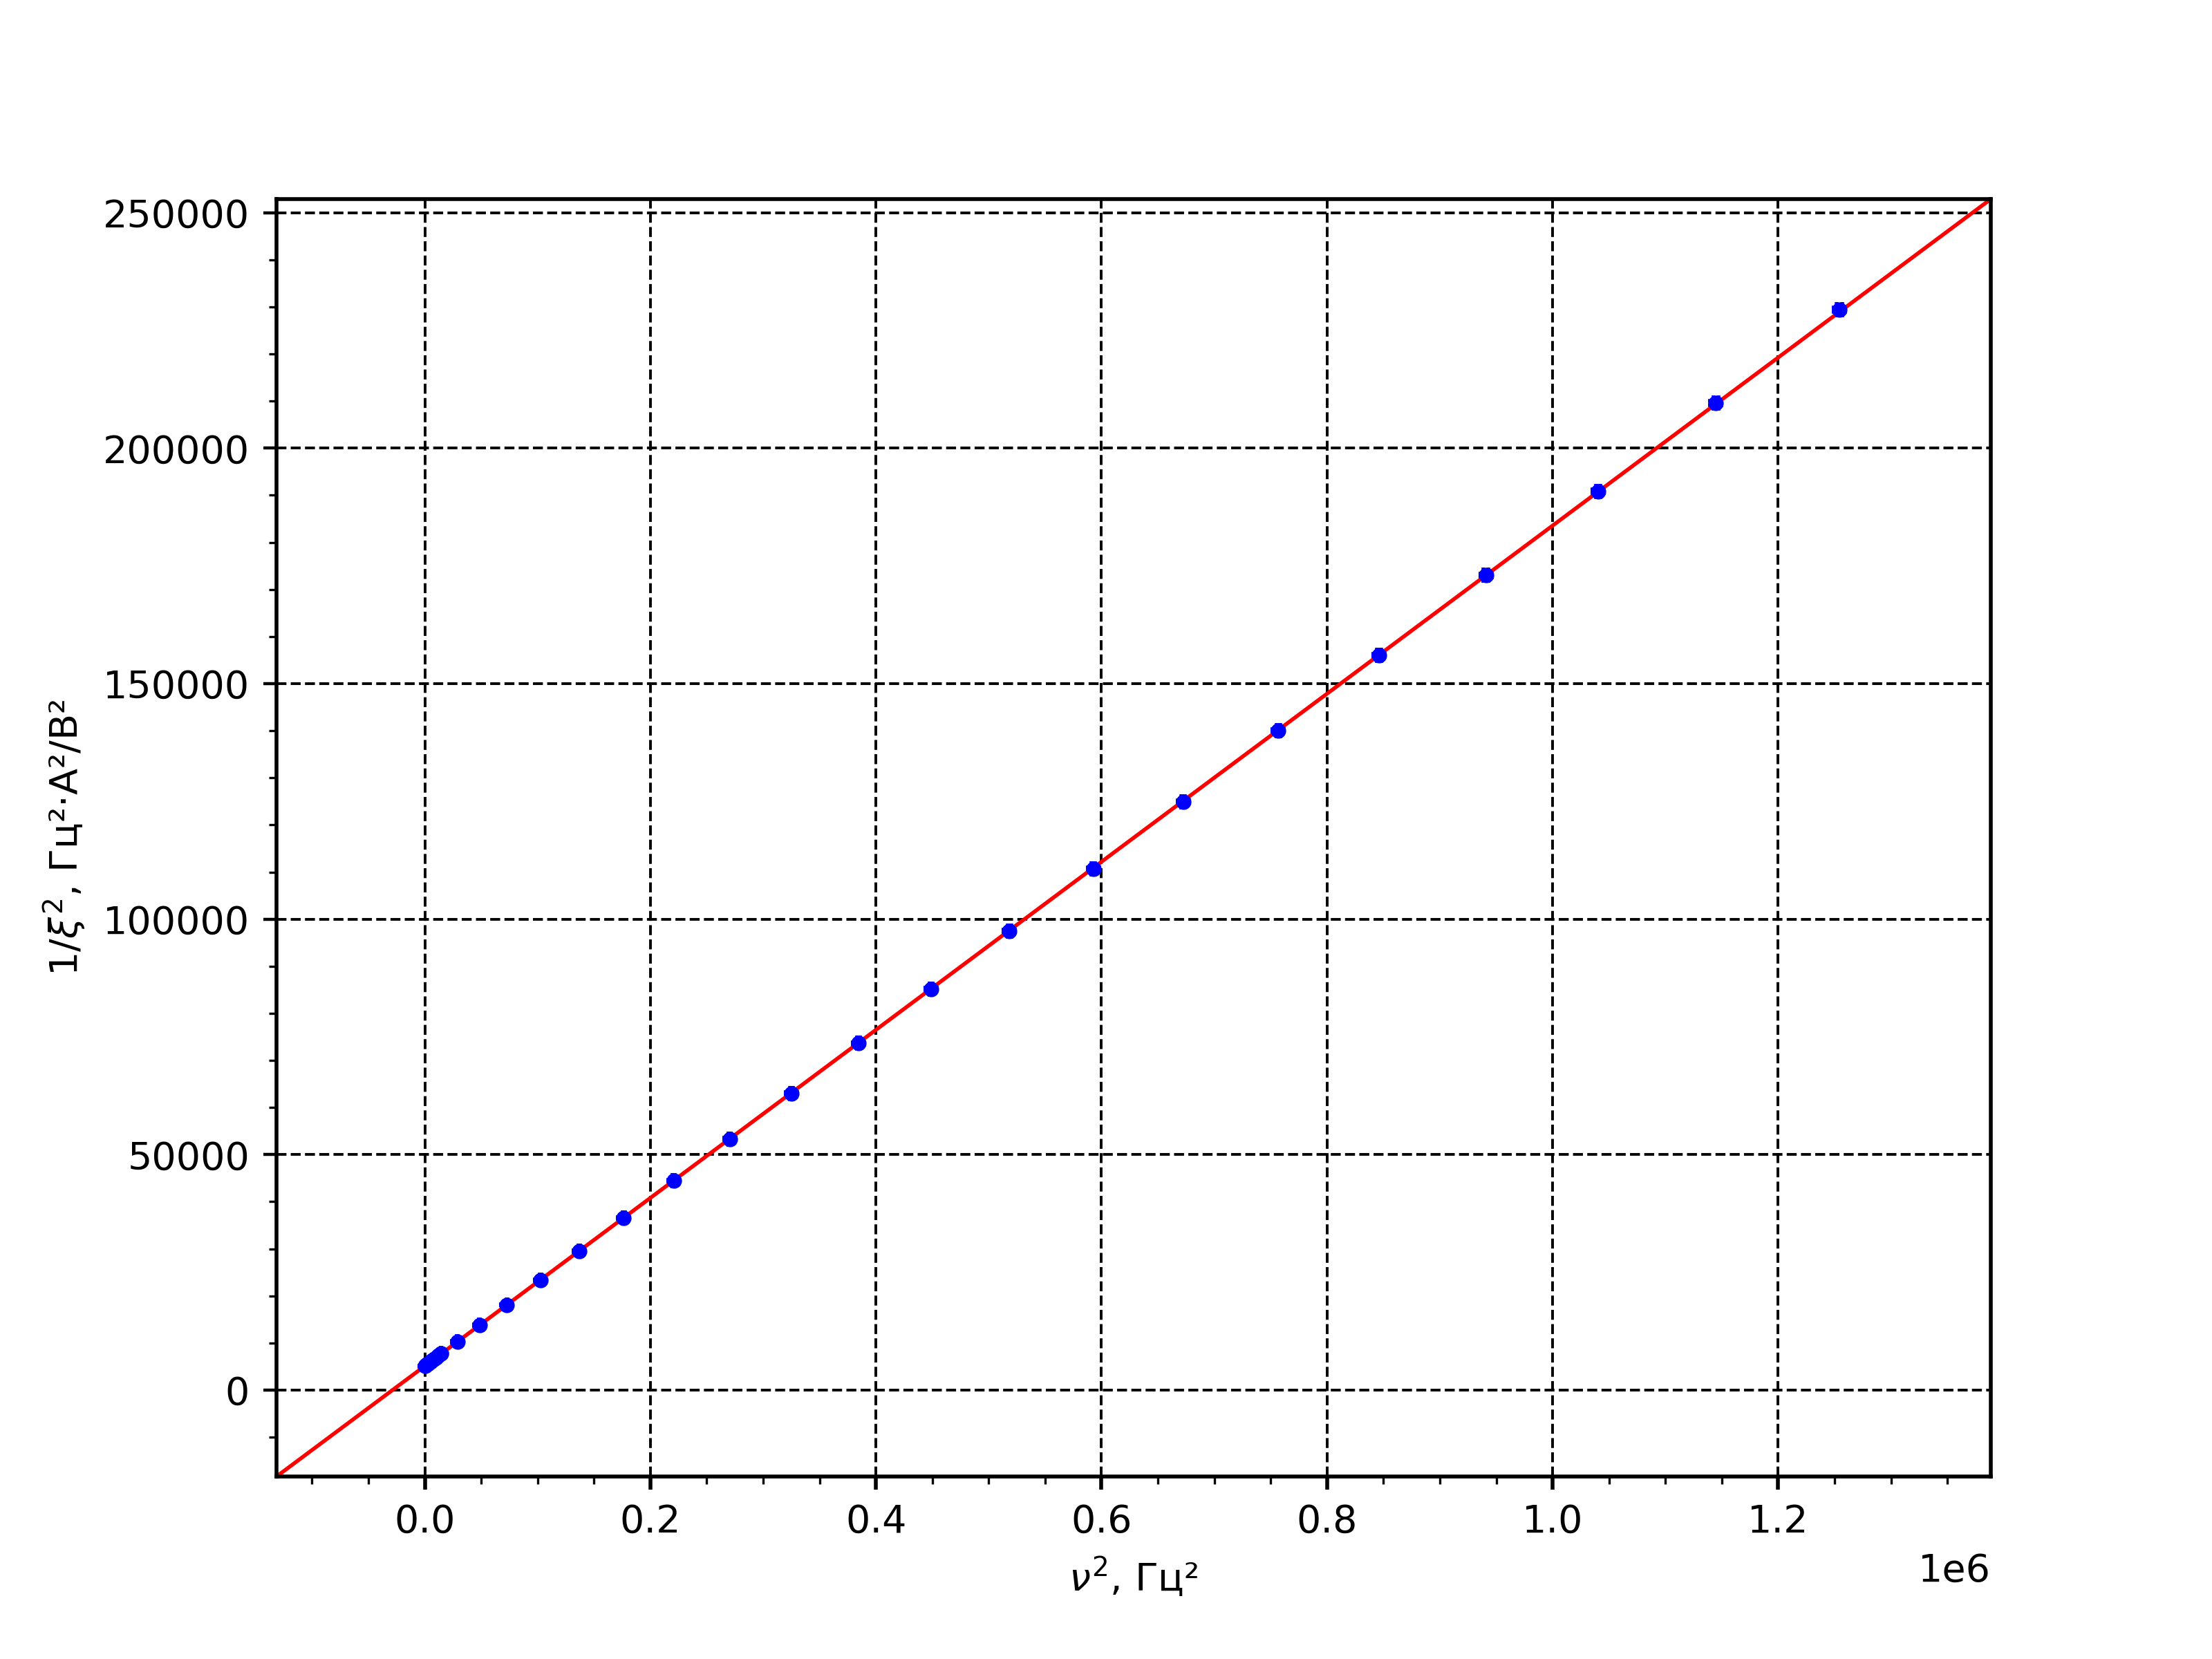
\includegraphics[width=0.8\linewidth]{../img/plot7.png}}
\end{figure}

\[
    b = 5116 \pm 4\;\text{Гц}^{2}\cdot\text{А}^{2} / \text{В}^{2}
\]

\[
    k = \left(17844 \pm 9\right)\cdot 10^{-5}\;\text{А}^{2} / \text{В}^{2}
\]

\[
    \xi_0 = \sqrt{1/b} =  \left(13981 \pm 6\right)\cdot 10^{-6}\;\text{В} / \text{Гц}\cdot\text{А}
\]

\[
    \sigma = \frac{\sqrt{k/b}}{\pi ah \mu_0} = \left(4432 \pm 2\right)\cdot 10^{4}\;\text{См} / \text{м}
\]
\begin{figure}[ht!]
    \center{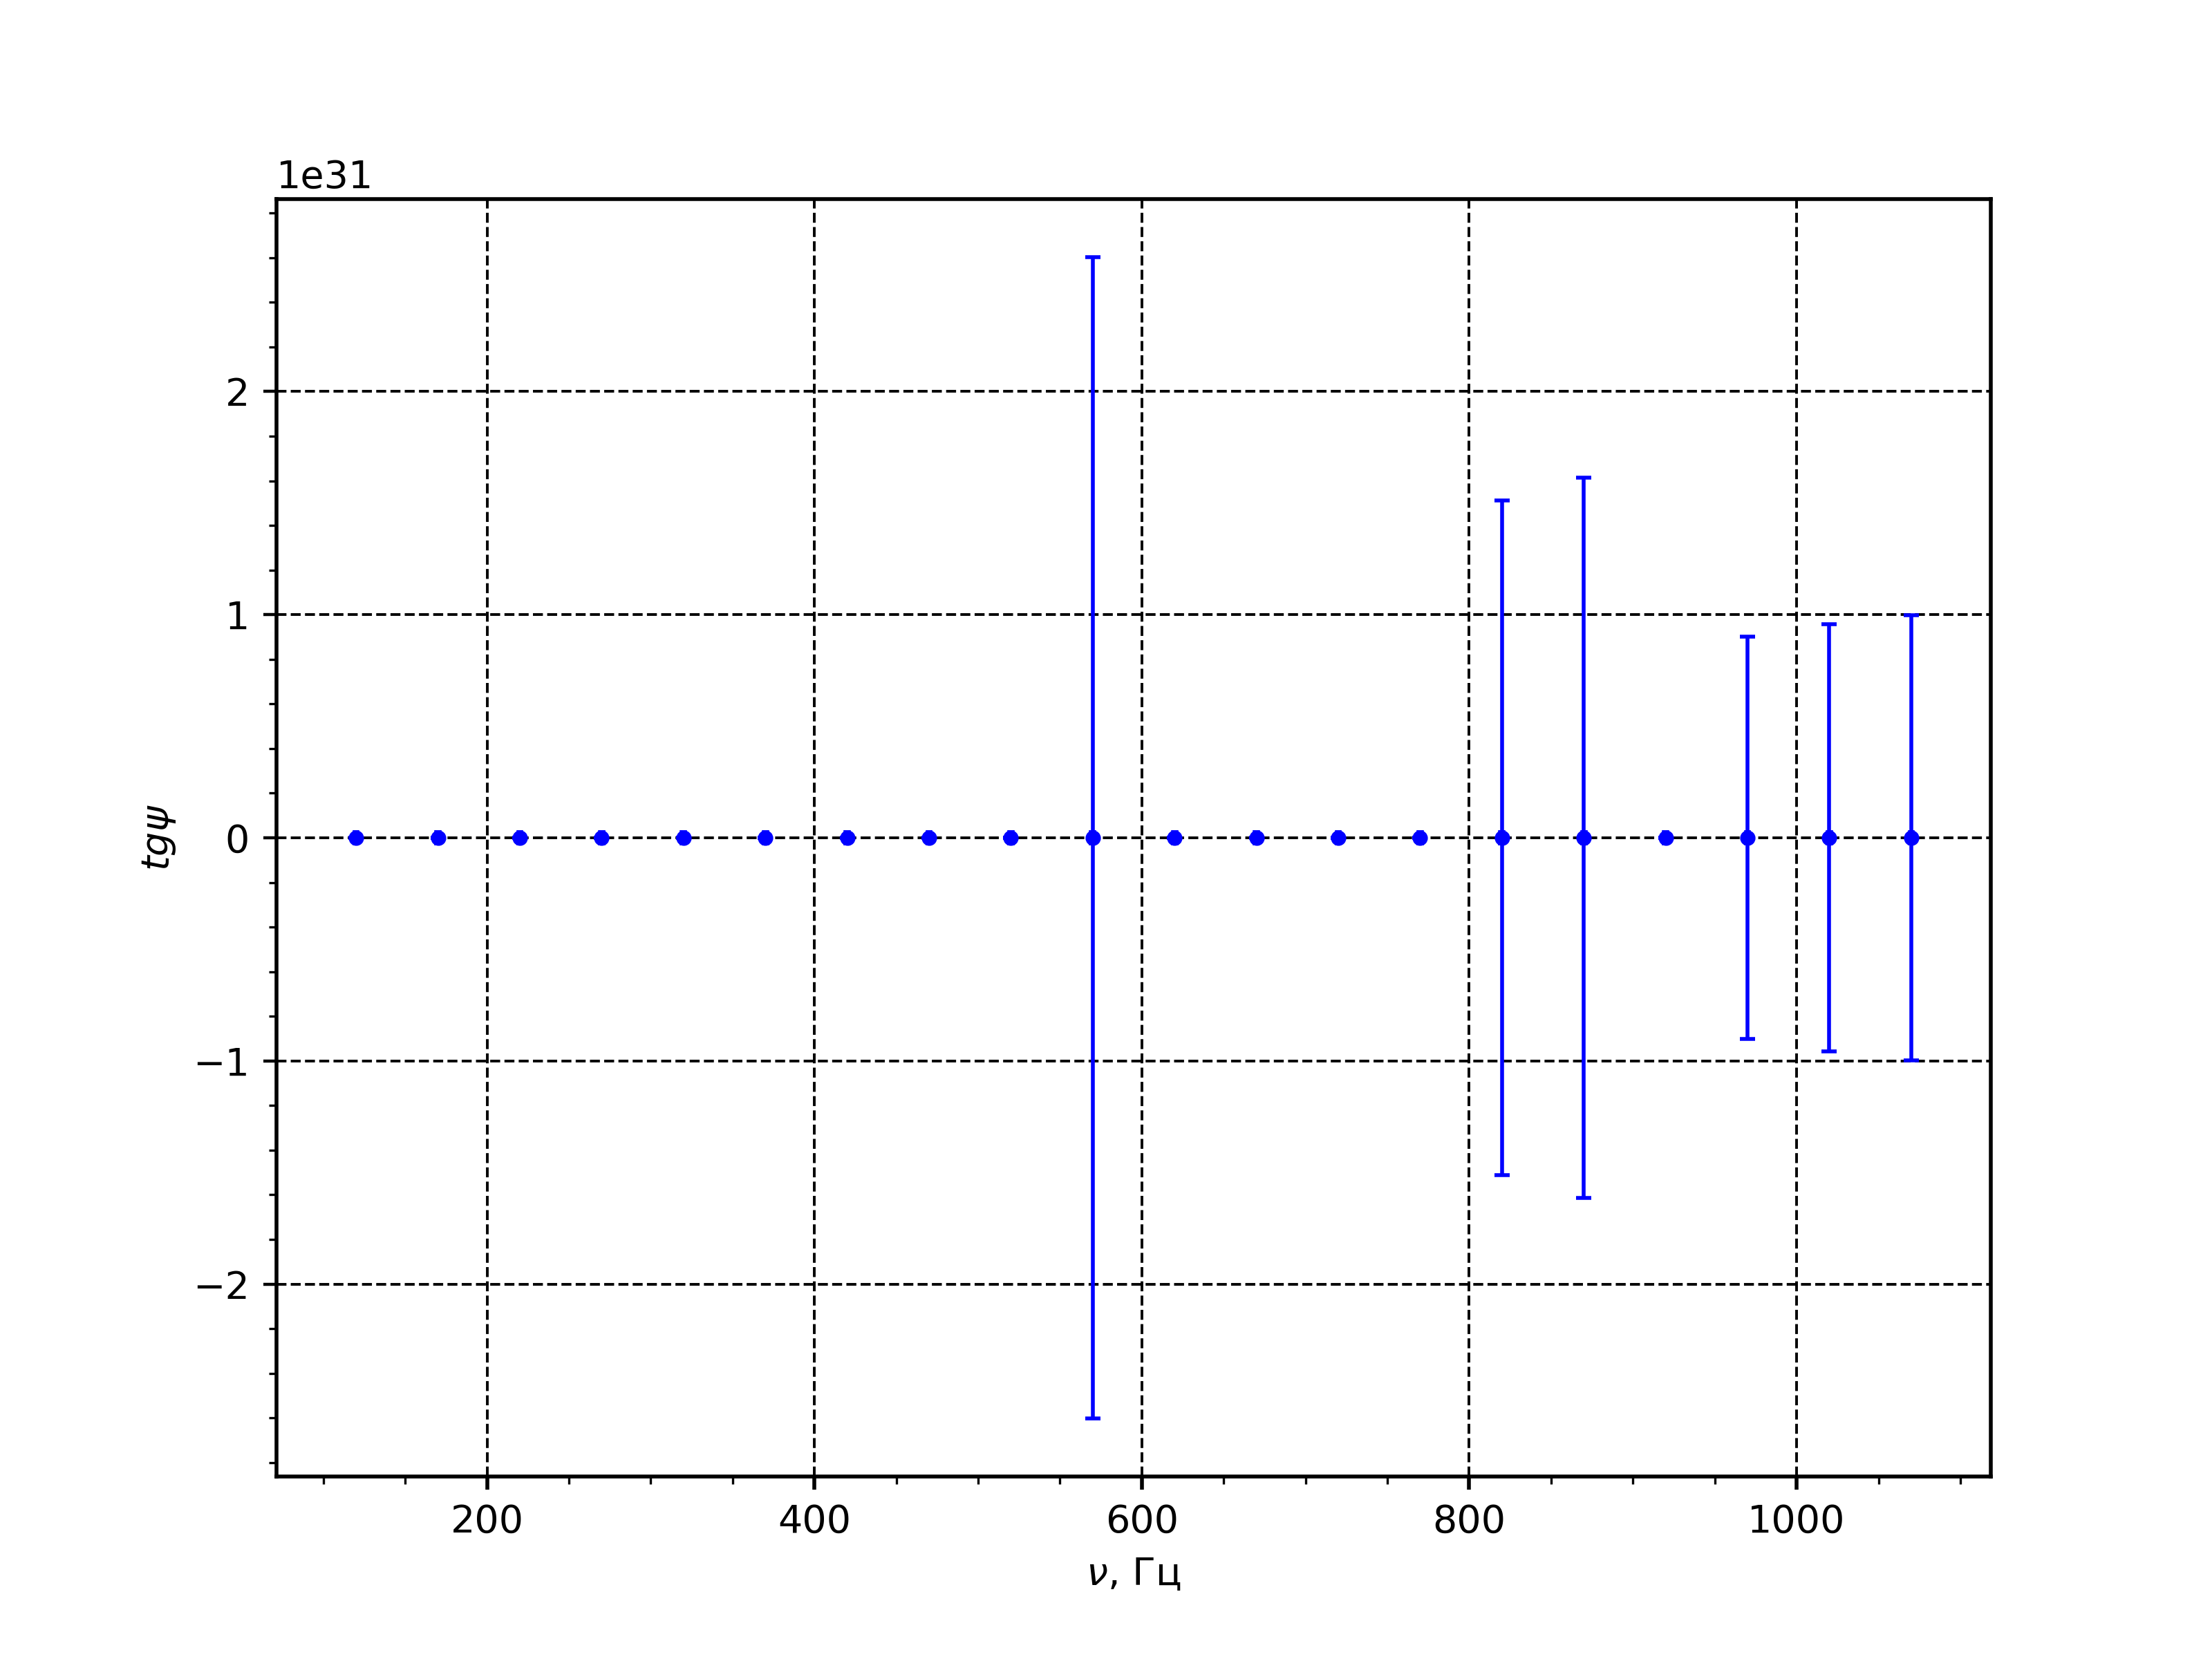
\includegraphics[width=0.8\linewidth]{../img/plot8_1.png}}
\end{figure}
\begin{figure}[ht!]
    \center{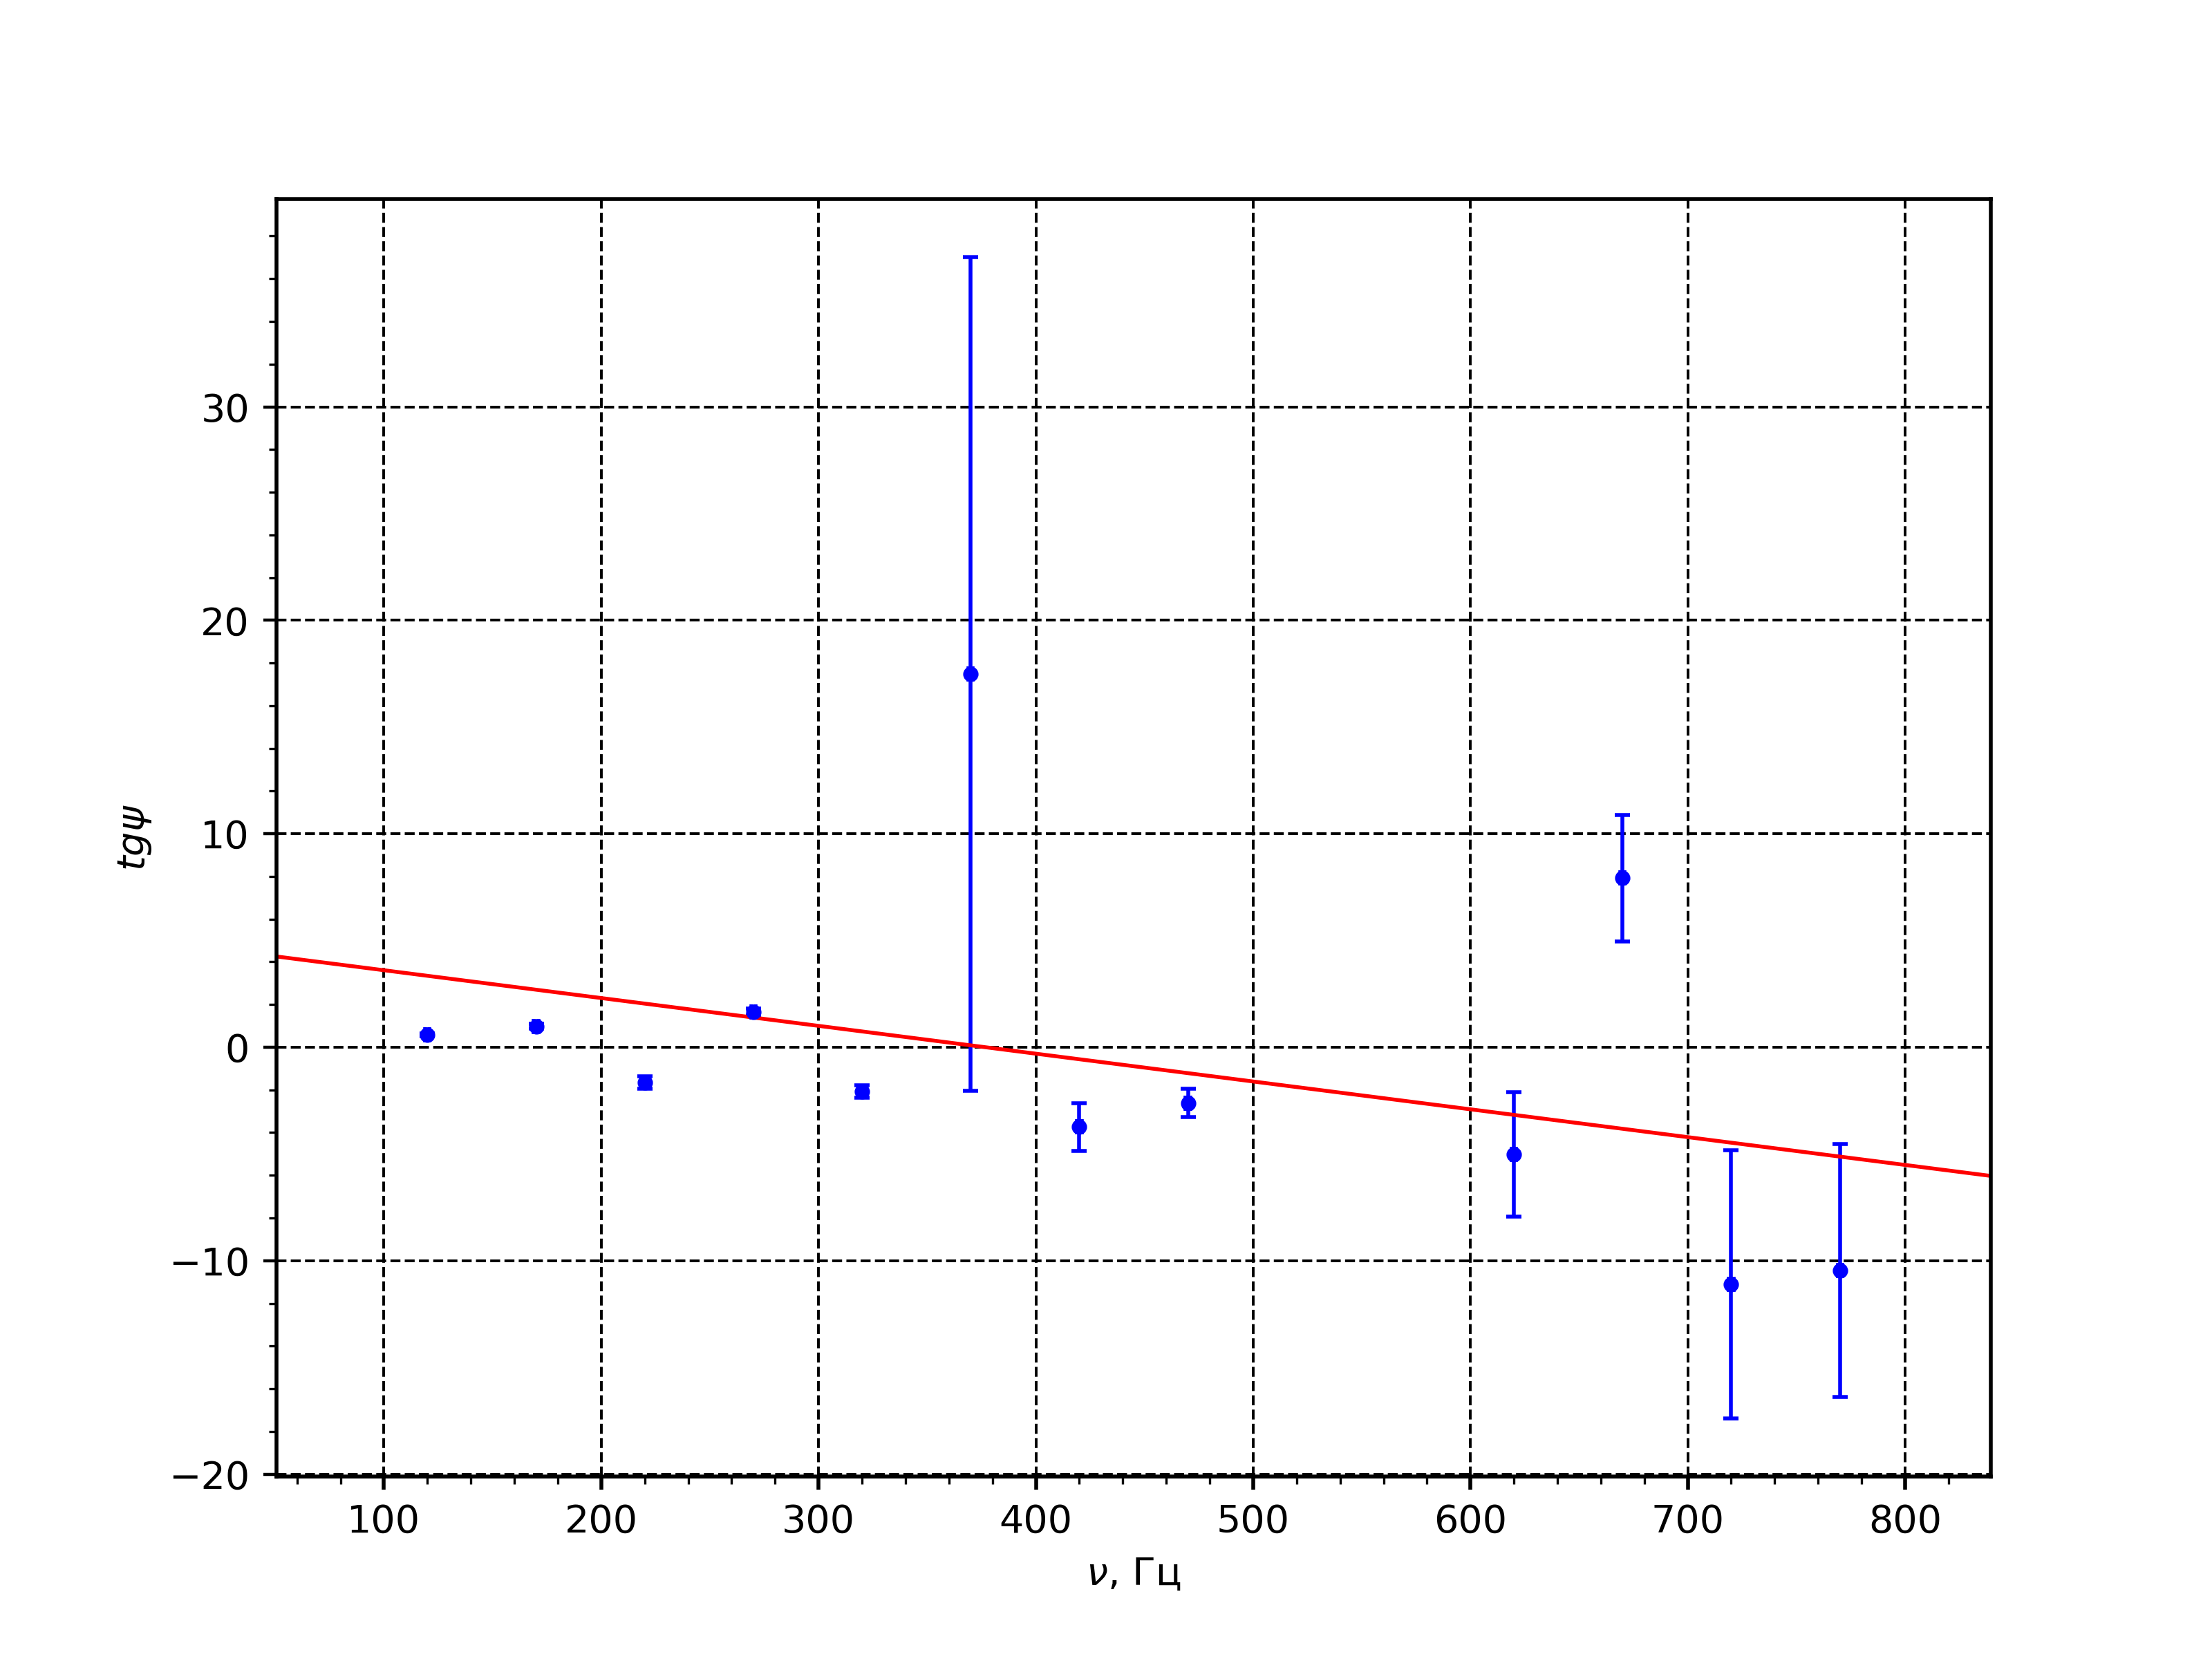
\includegraphics[width=0.8\linewidth]{../img/plot8_2.png}}
\end{figure}

\[
    k = \left(-7 \pm 7\right)\cdot 10^{-3}\;\text{Гц}^{-1}
\]

\[
    \sigma = \frac{2k}{ah\mu_0} = \left(-3 \pm 3\right)\cdot 10^{8}\;\text{См} / \text{м}
\]

Значение сильно отличается от истины и погрешность велика, т.к. погрешность тангенса сильно растет при приближении к $\pi$, а также
точности определения разности фаз осциллографом не хватает.

\begin{figure}[ht!]
    \center{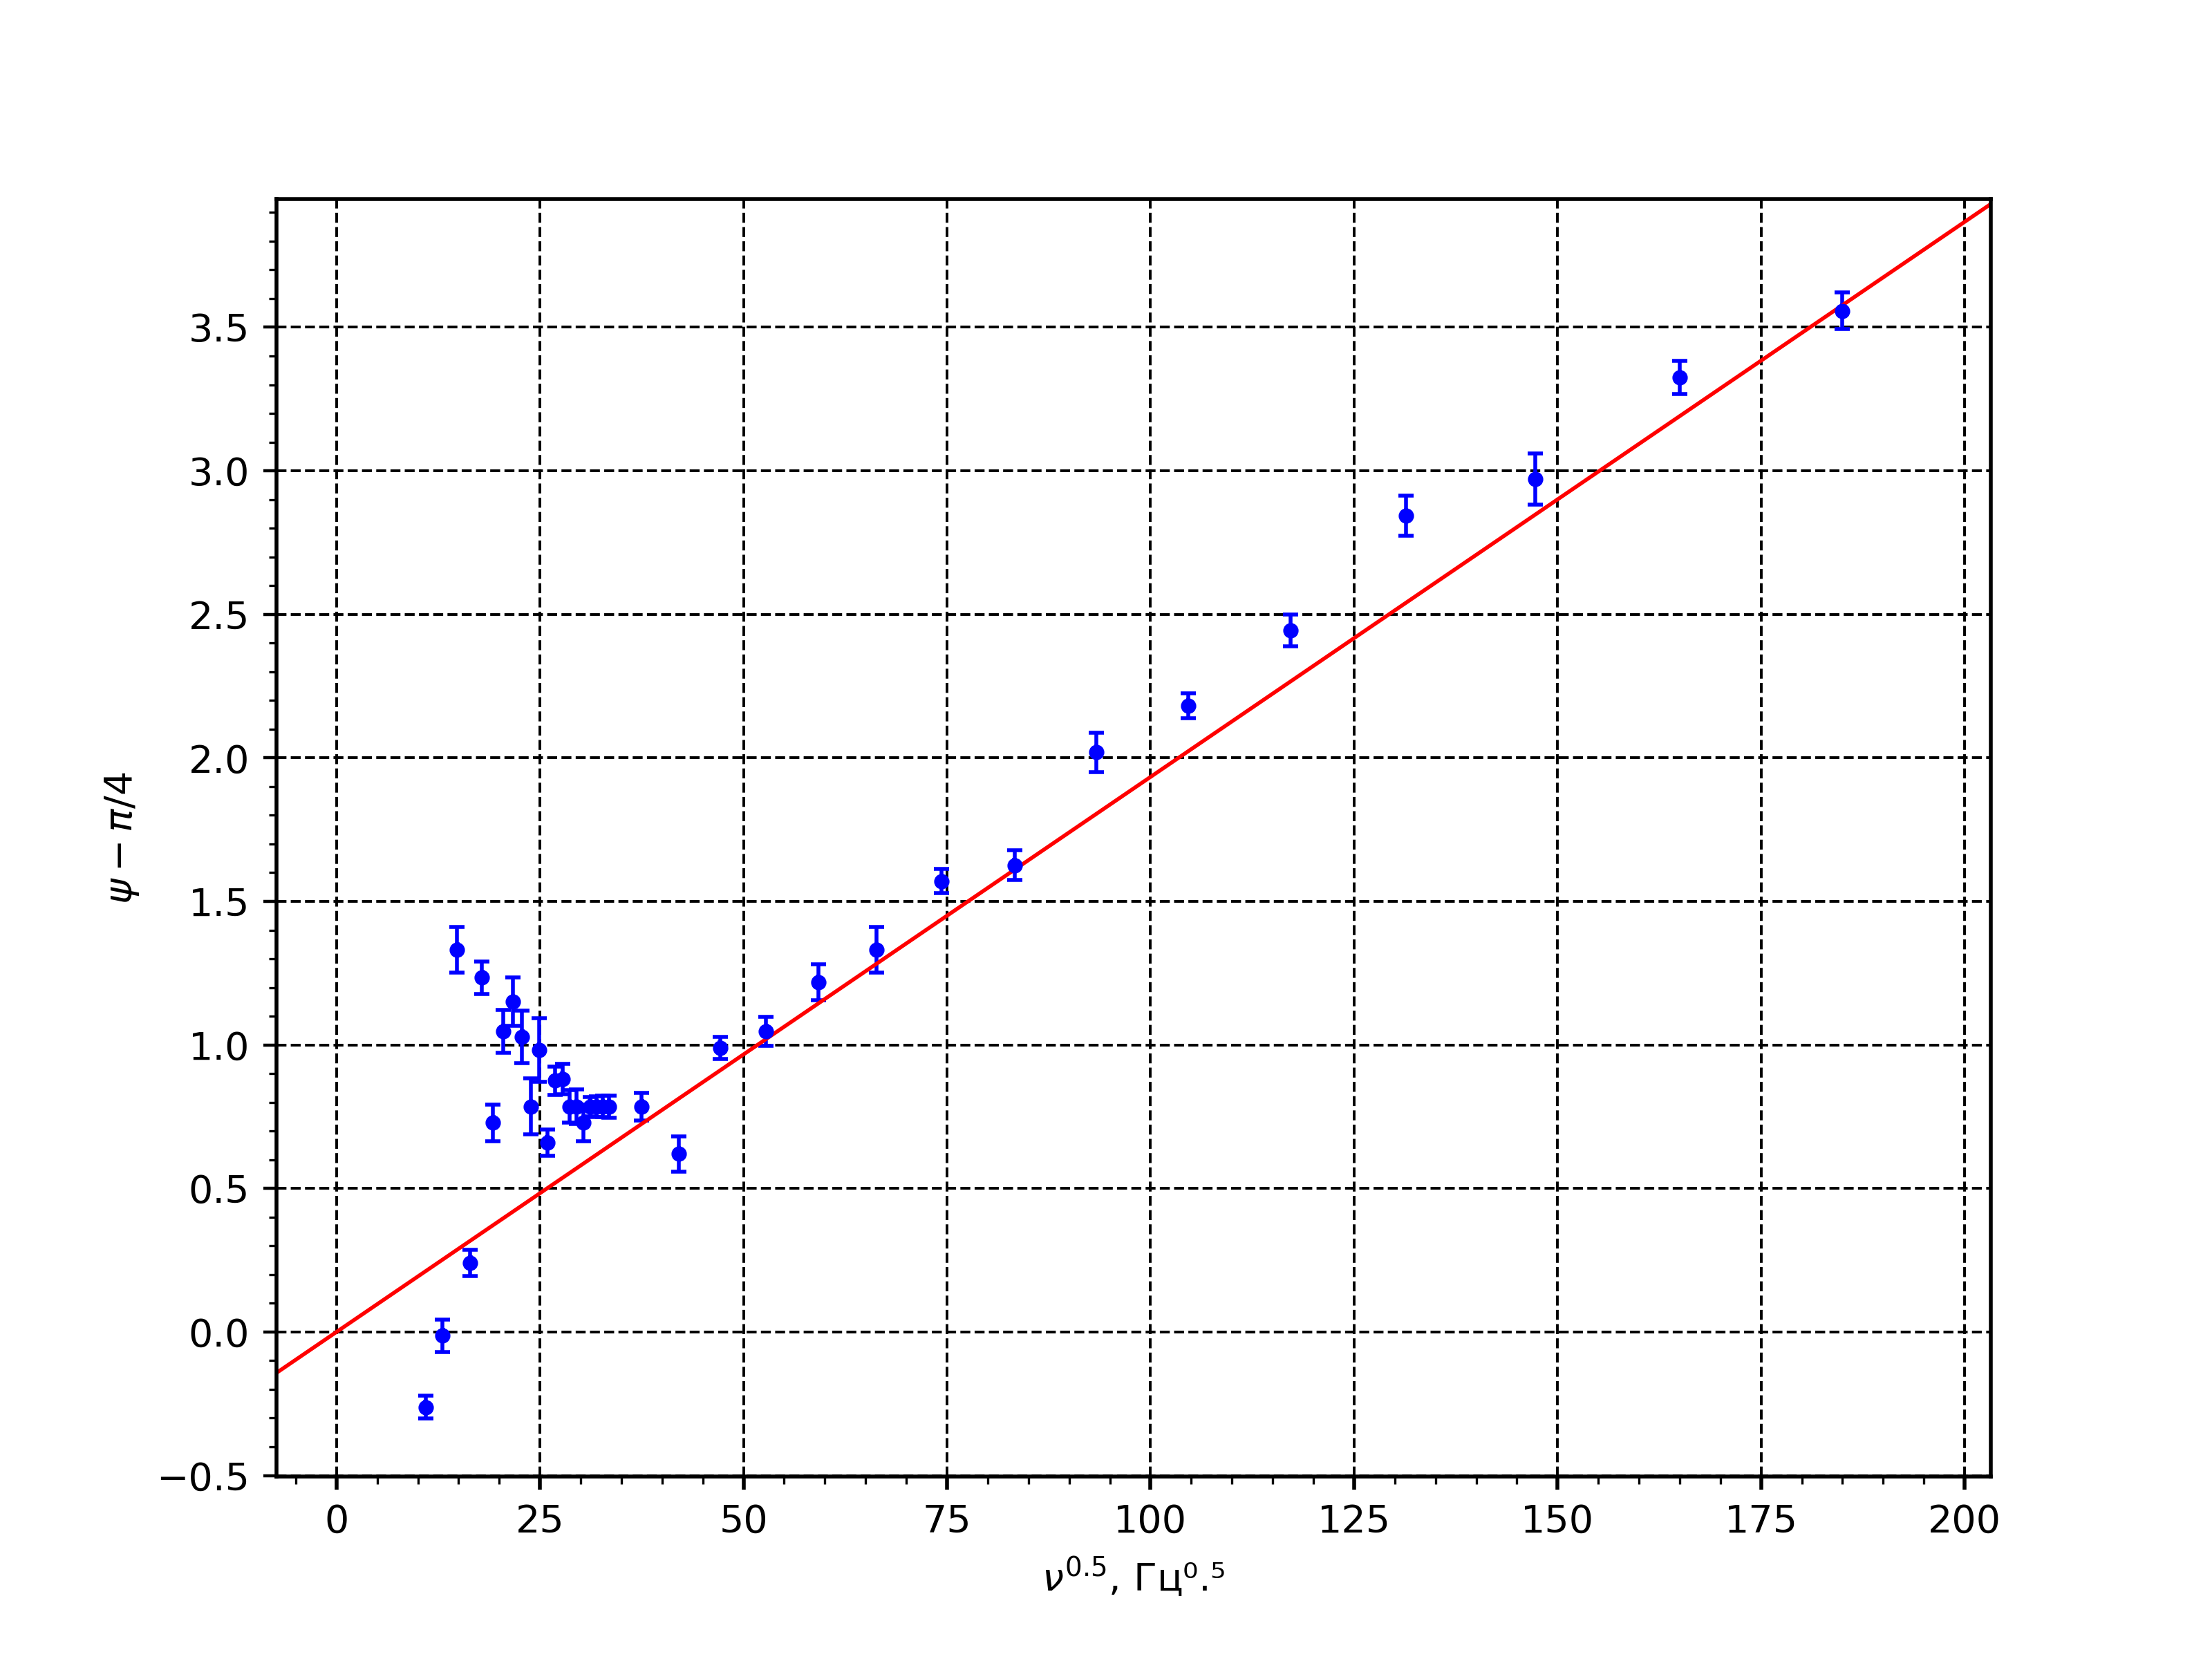
\includegraphics[width=0.8\linewidth]{../img/plot9.png}}
\end{figure}

\[
    k = \left(193 \pm 7\right)\cdot 10^{-4}\;\text{Гц}^{-0.5}
\]

\[
    \sigma = \frac{k^2}{h^2 \pi\mu_0} = \left(42 \pm 3\right)\cdot 10^{6}\;\text{См} / \text{м}
\]

\begin{figure}[ht!]
    \center{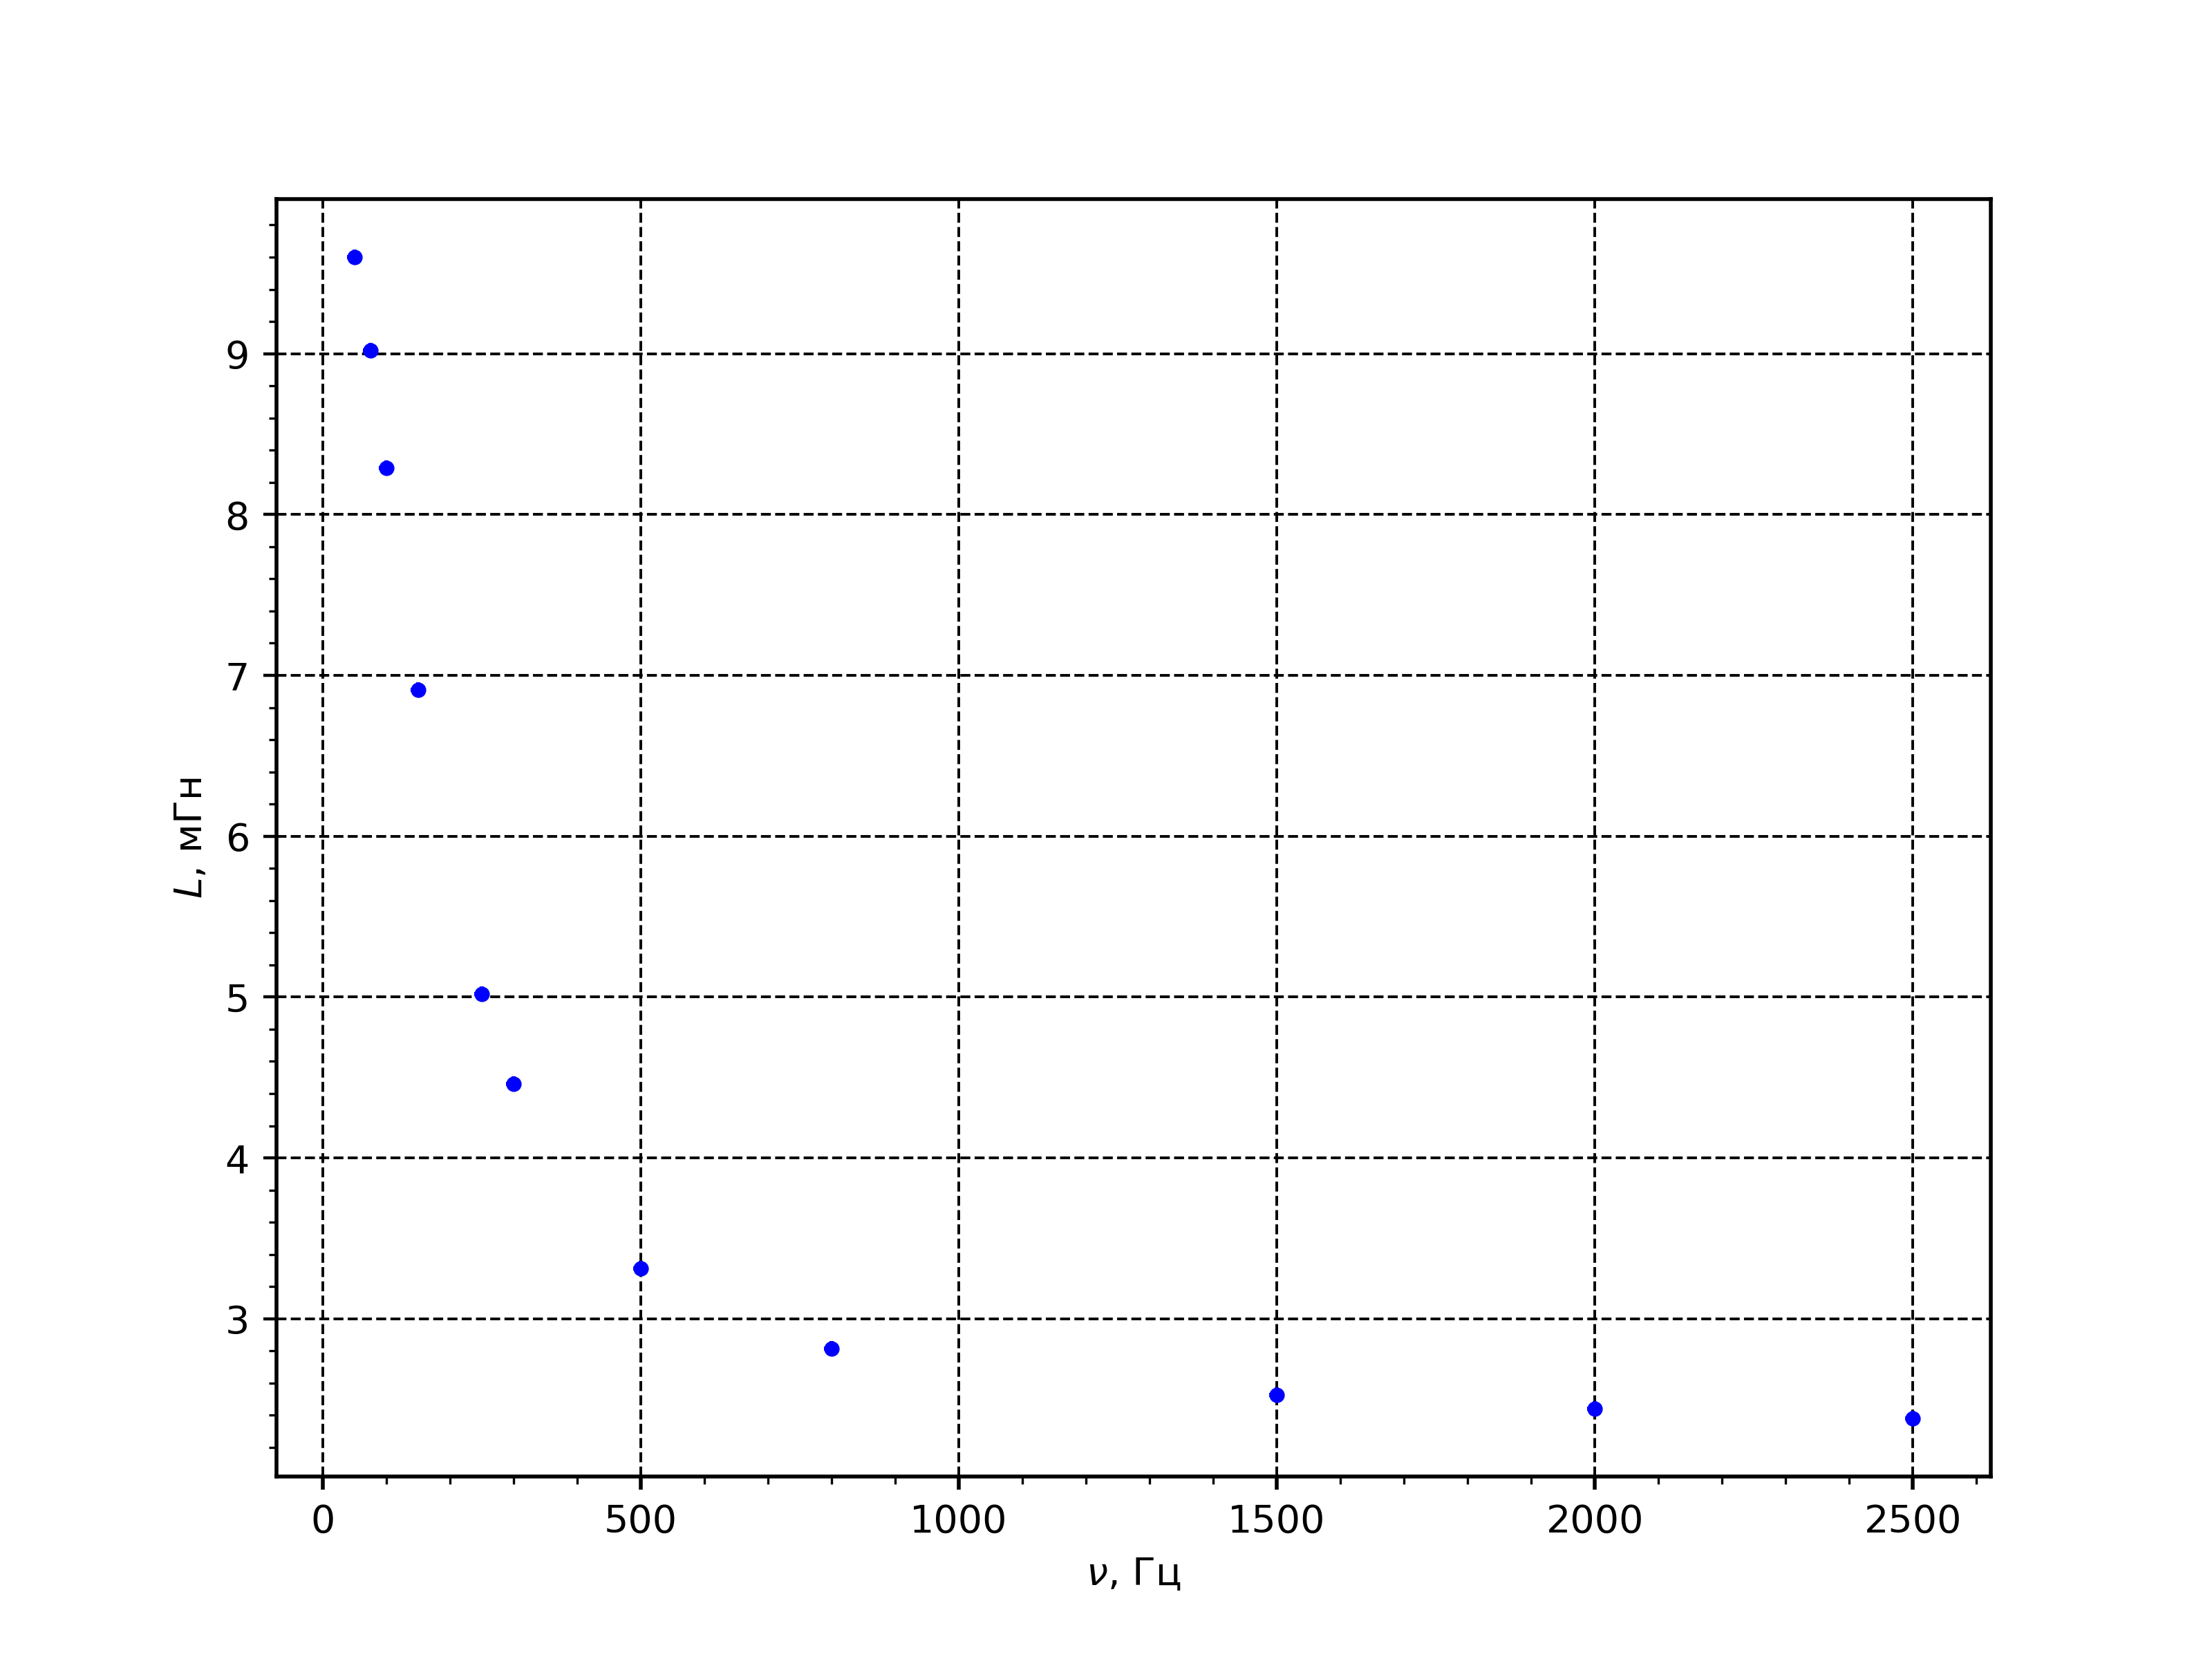
\includegraphics[width=0.8\linewidth]{../img/plot10-1.png}}
\end{figure}
\begin{figure}[ht!]
    \center{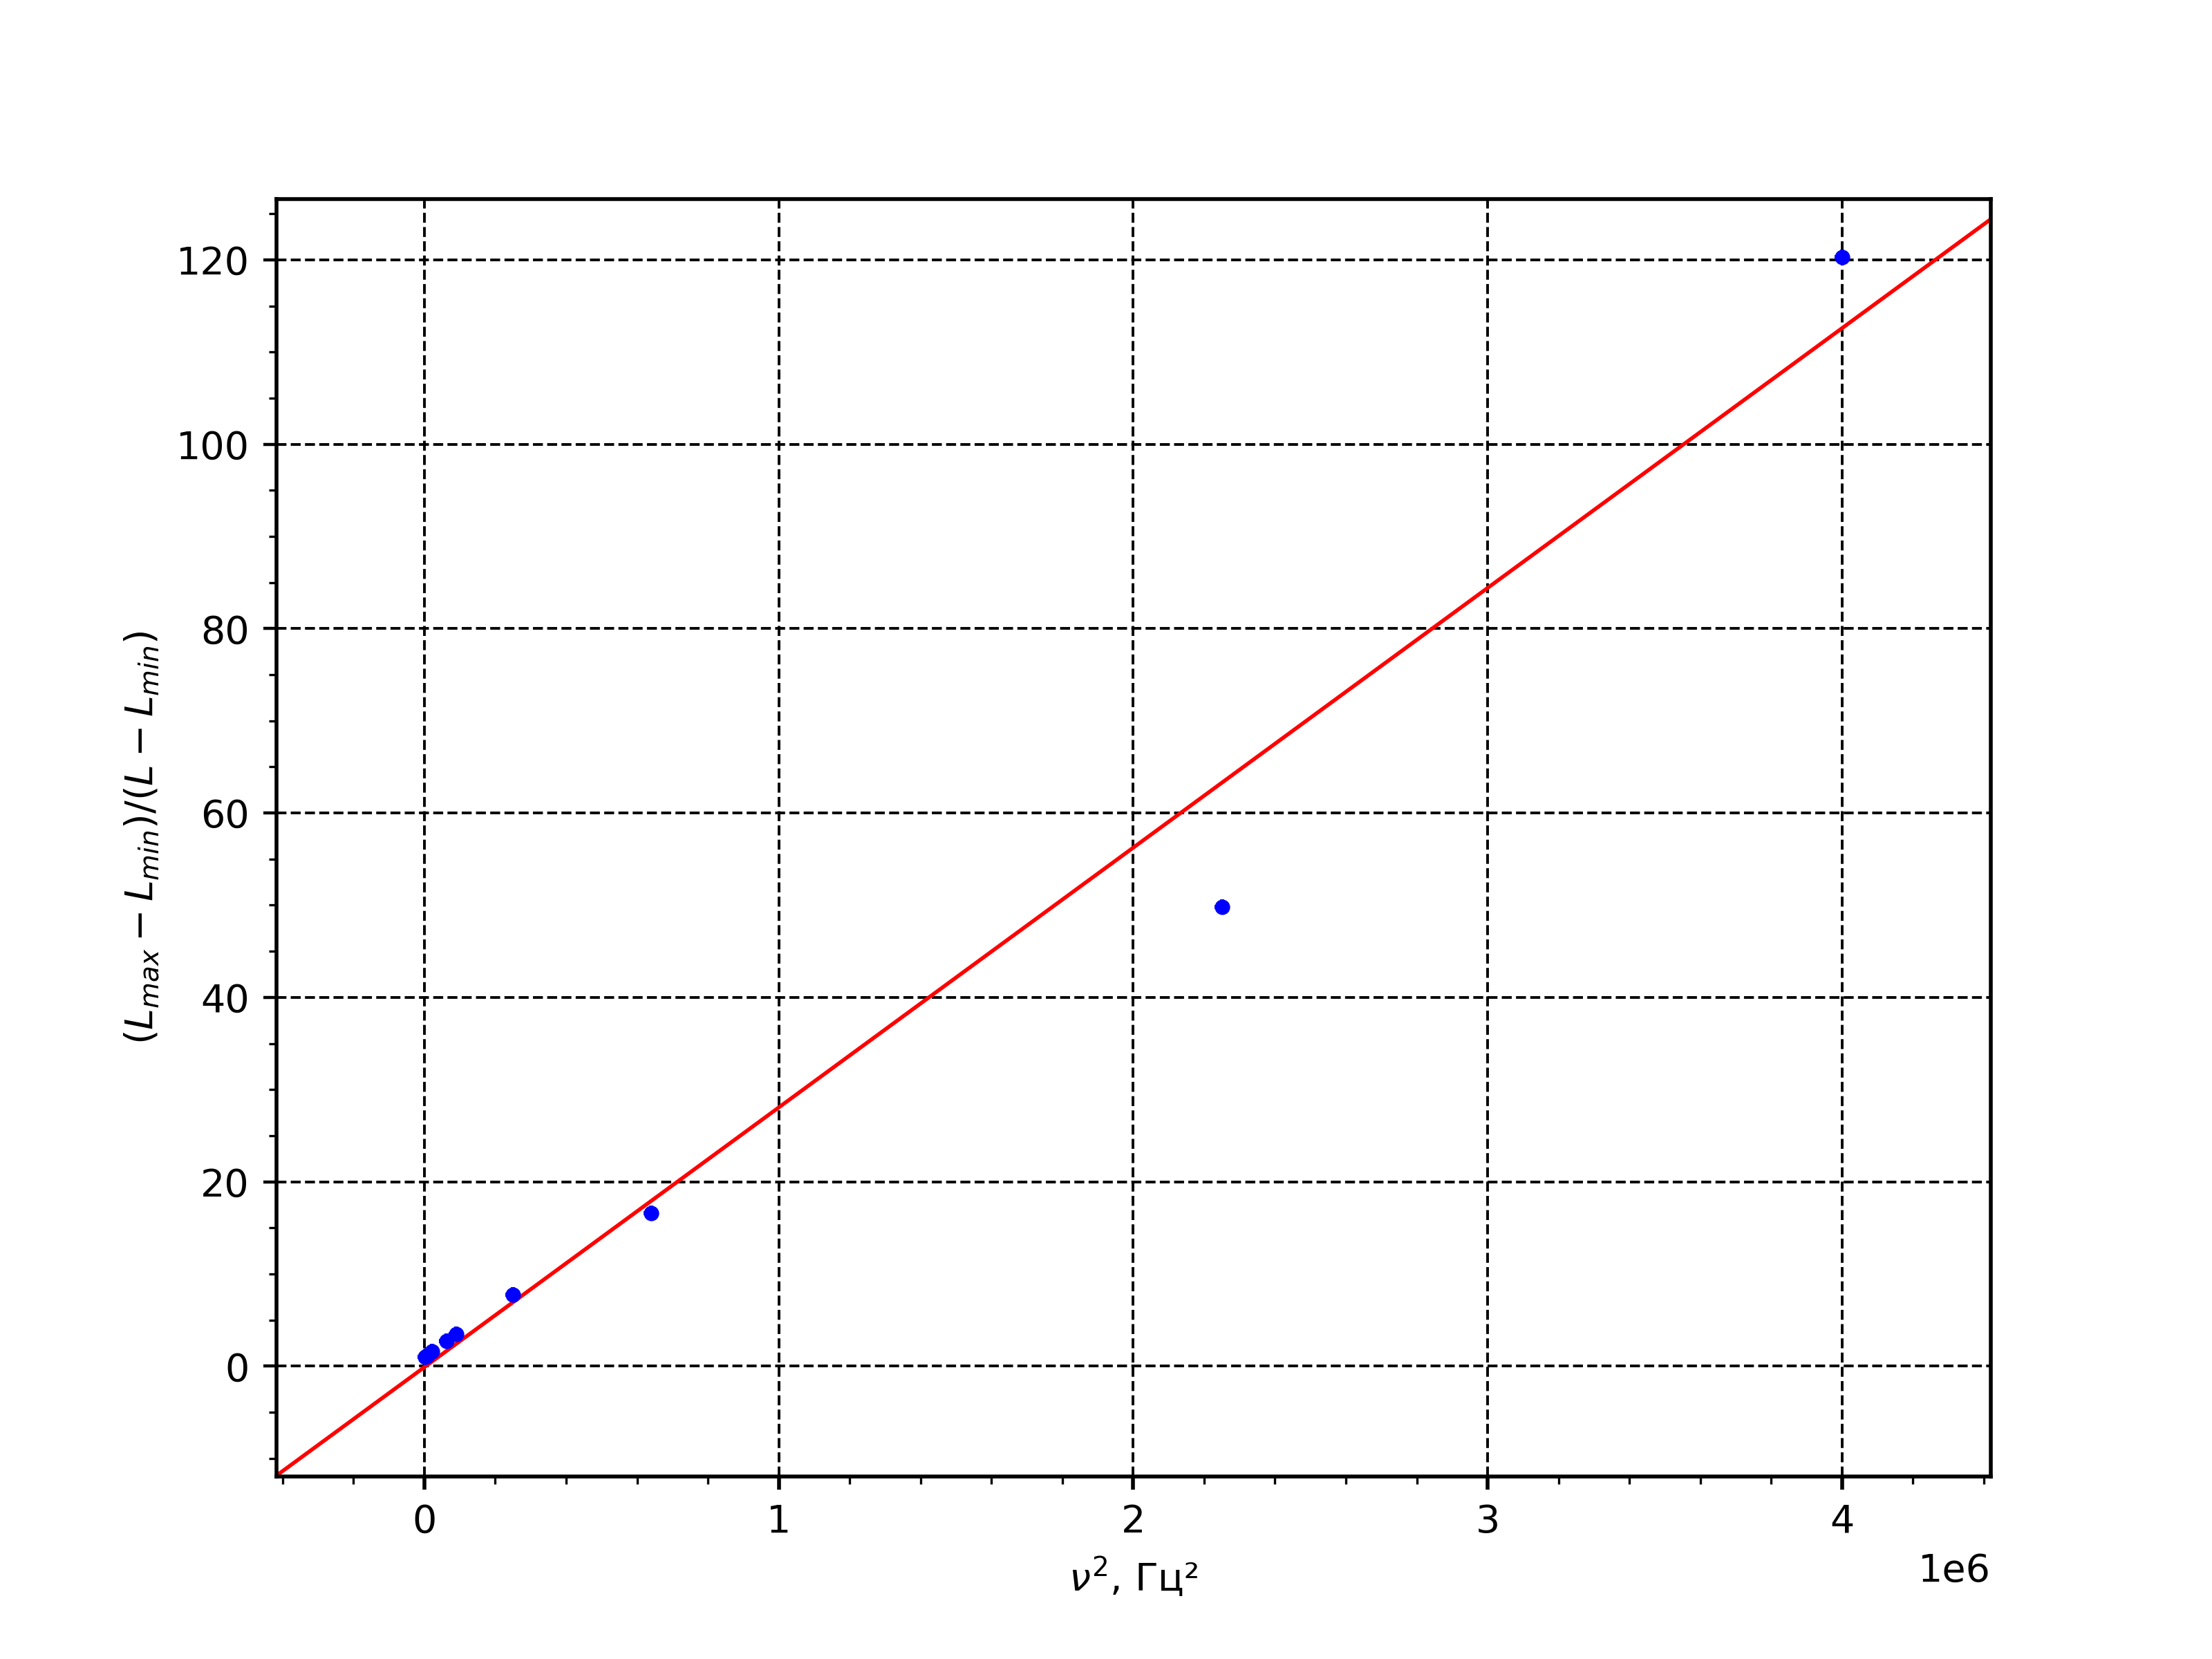
\includegraphics[width=0.8\linewidth]{../img/plot10-2.png}}
\end{figure}

\[
    L_{max} = 9{,}6\;\text{мГн}\;\;\; L_{min} = 2{,}38\;\text{мГн}
\]

\[
    k = \left(28{,}2 \pm 1{,}4\right)\cdot 10^{-6}\;\text{Гц}^{-2}
\]

\[
    \sigma = \frac{\sqrt{k}}{\pi ah \mu_0} = \left(39{,}8 \pm 1{,}0\right)\cdot 10^{6}\;\text{См} / \text{м}
\]

\[
    \sigma_0 = 5{,}9\cdot 10^7\;\text{См}/\text{м}
\]
\begin{figure}[ht!]
    \center{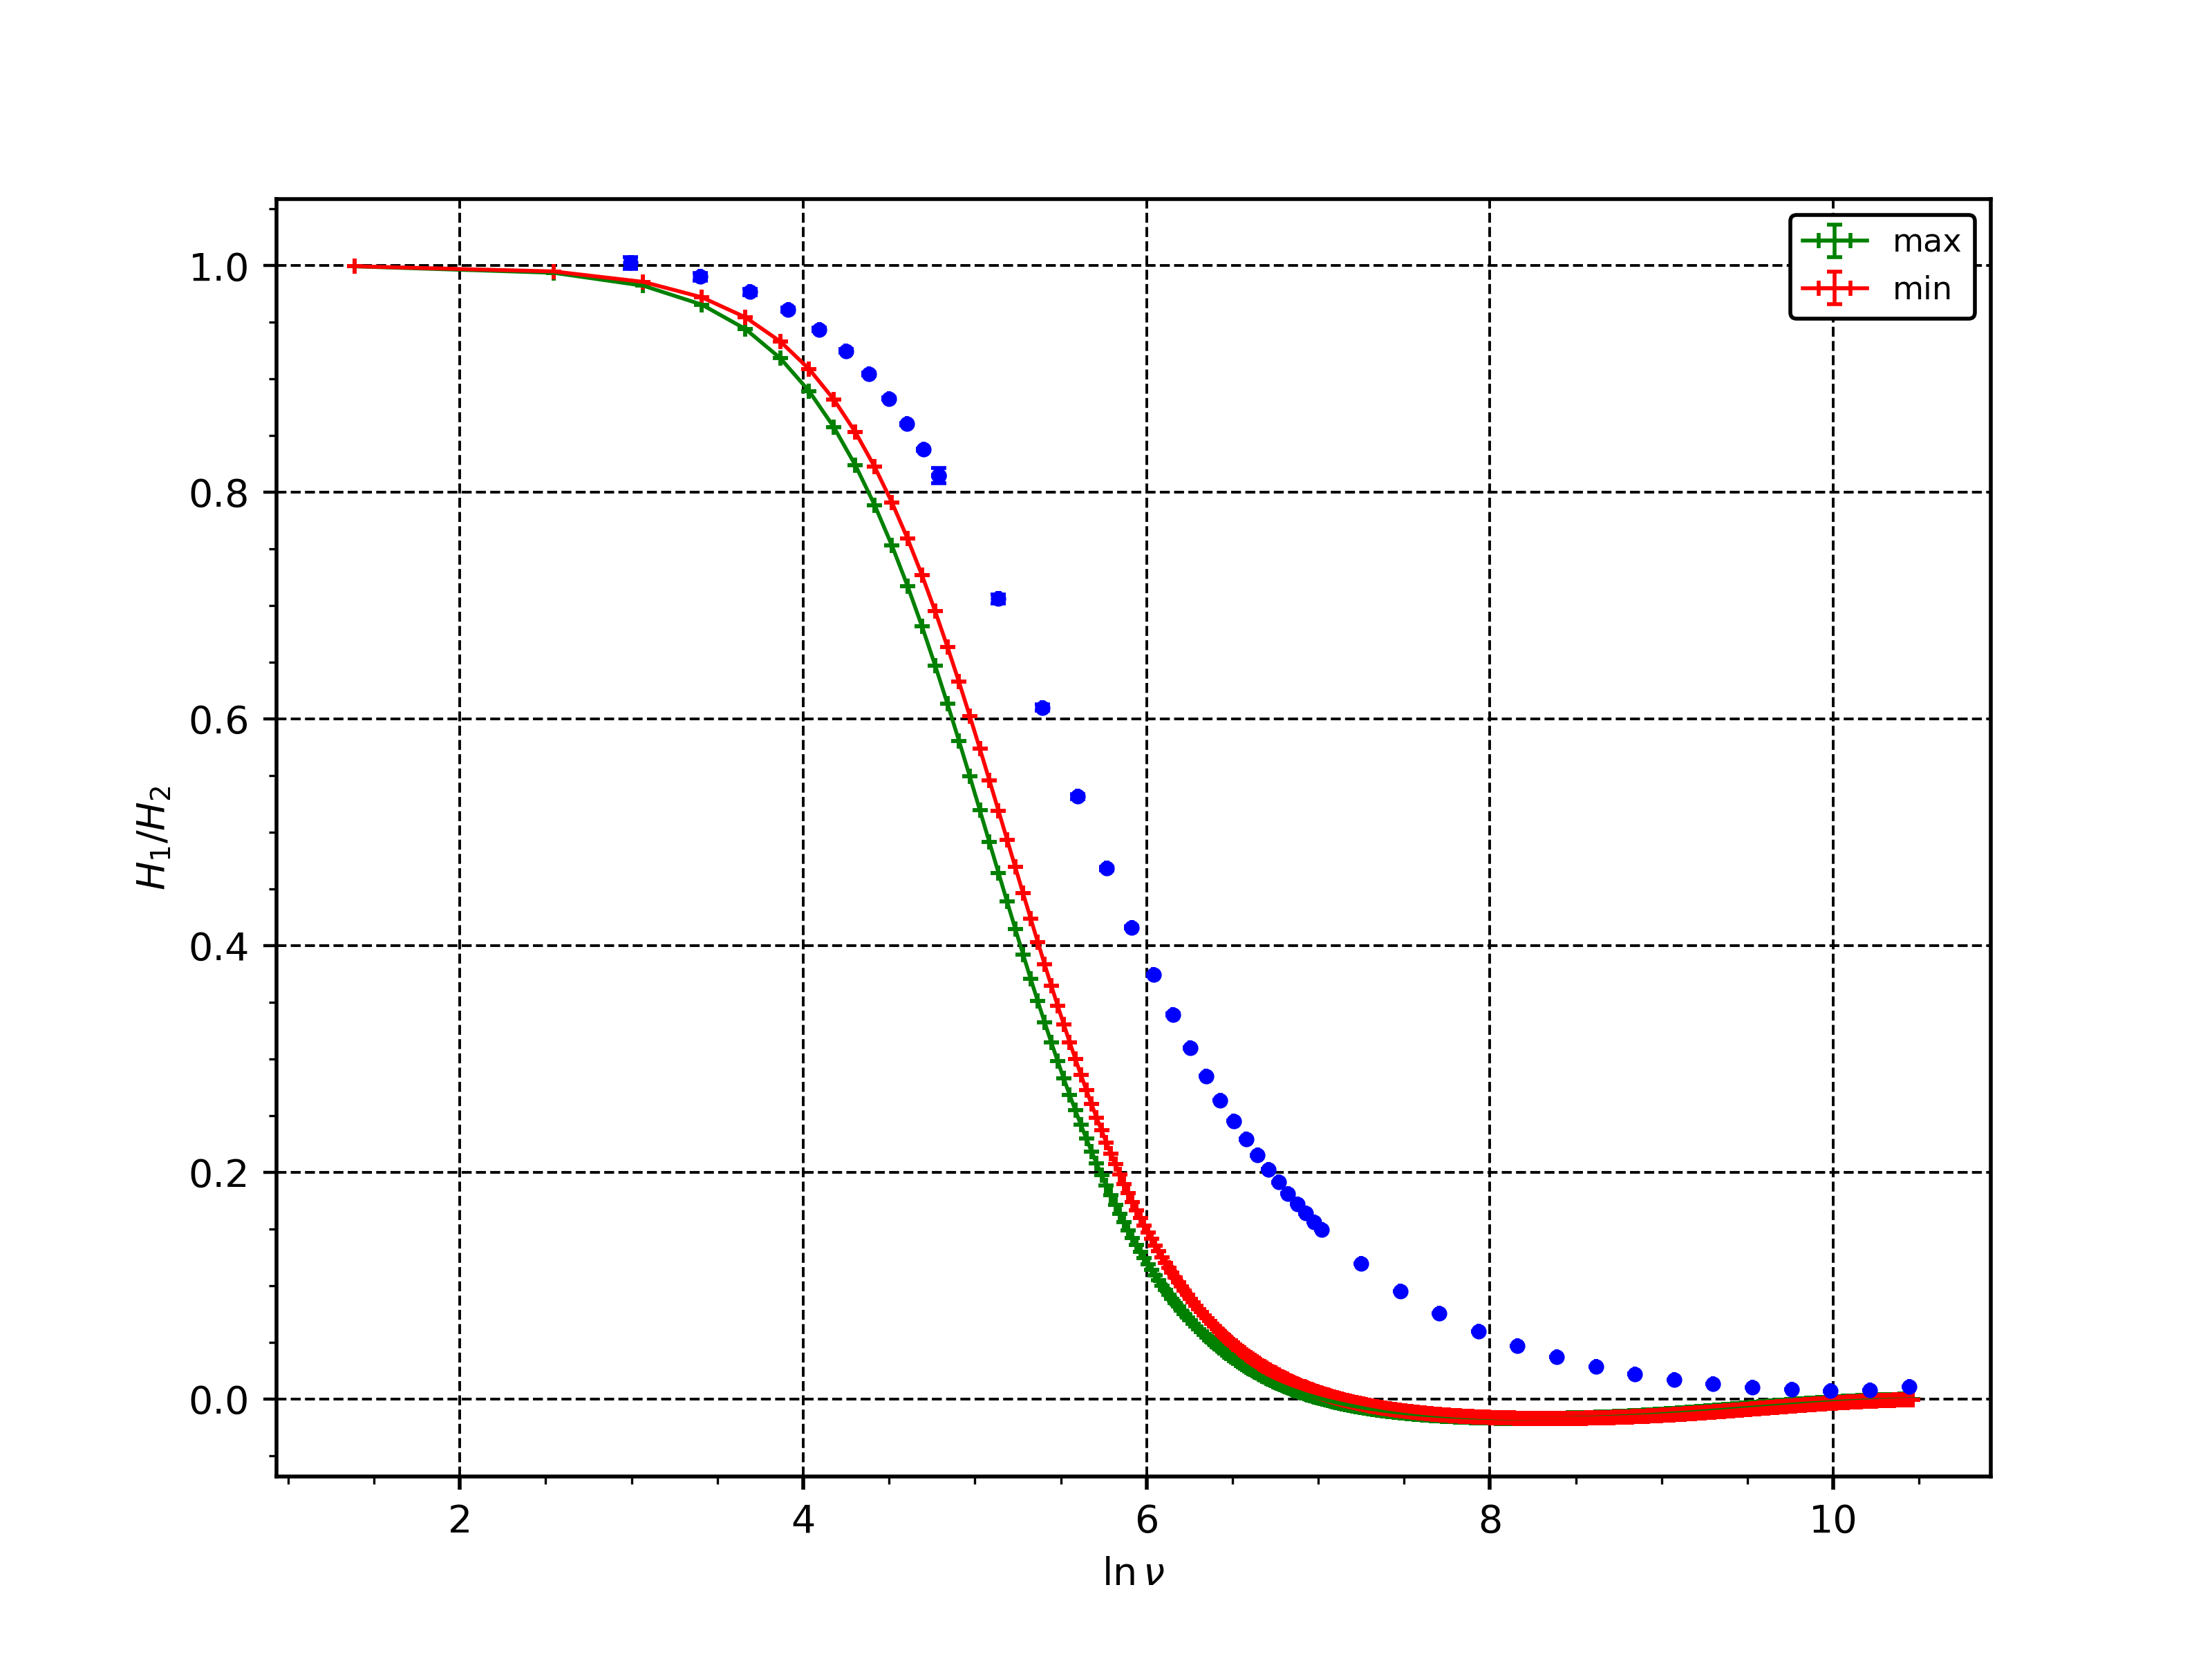
\includegraphics[width=0.8\linewidth]{../img/plot12.png}}
\end{figure}

